\chapter{X-WikiRE}
\label{chpt:4}
\paragraph{}
In this chapter we will describe how we built \textbf{X-WikiRE}. We will start by describing the datasources used, Wikipedia and Wikidata. Next, we will describe the process we used to combine these resources to obtain automatically annotated data for different languages. As final step, we will describe how to increase the number of examples by creating different templates. In the last section, we will show some descriptive statistics about \textbf{X-WikiRE}.

\section{Introduction}
\paragraph{}
Supervised training of deep neural networks often requires large amounts of high-quality training data which are difficult to obtain.  To fix this, ~\cite{hewlett2016wikireading} exploited Wikidata~\citep{vwikidata} and Wikipedia to create large amounts of distantly annotated data for various natural understanding tasks. \cite{levy2017zero} use WikiReading as a starting point for building a large scale reading-comprehension based dataset for relation extraction. Based on these two works we build \textbf{X-WikiRE}, a new large scale multilingual reading-comprehension based dataset for relation extraction. \textbf{X-WikiRE} is available in English, Spanish, Italian, German, and French, and is also on at least a magnitude order larger than other multilingual resources for RE.

\section{Datasources}
\paragraph{}
Our datasources are Wikipedia, and Wikidata. Wikidata it is a free collaborative knowledge base that is available in more than 300 languages. Its value has long been obvious, with many efforts to use it. The Wikidata approach is to crowd source data acquisition, allowing a global community to edit it's content, making it a good quality resource.  Wikipedia is a online encyclopedia with articles available, as for Wikidata, in more than 300 languages. Wikipedia consists of textual articles describing entities. %Wikidata provides dumps in different data formats, spanning from XML, Turtle, NTriples, and JSON. We choose the latter and describe below it's datamodel. Instead Wikipedia only provides XML dumps, which can be converted to JSON using existing tools\footnote{\url{https://www.mediawiki.org/wiki/Alternative_parsers}}, but we opted to scrape them since the output provided by these tools is sometimes too noisy or require some changes to allow the merge with Wikidata.

% The two used sources are are different in both size, and contained information. We can have a quick recap in Table~\ref{tab:datasets}. The next two sections will present a more in detail description of these resources.

% TODO ADD other languages stats.
% \begin{table}[h]
%     \centering
%     \begin{tabular}{l|l|l}
%          &  Wikidata & EN Wikipedia  \\ \hline
%     Documents  & 50M & 5.5M \\
%     Size & 730GB & 15GB \\
%     Information & Semi-structured & Unstructured \\
%     \end{tabular}
%     \caption{Dataset stats}
%     \label{tab:datasets}
% \end{table}

% \paragraph{Wikidata}
We can see Wikidata as a collection of triples \texttt{(entity\_id, property\_id, value)}. Each entity is identified by a unique number, prefixed with the letter Q, known as a ``QID". Also properties, which define the relation between the entities, are identified by a prefix P and a number (e.g. ``\texttt{P35}" is the id for the property \textit{``head\_of\_state"}). The relations each entity holds with other entities are called \textit{statements}, so a document corresponding to an entity, is a set of triples or statements. Values could be either other entities, or numeric/textual values.  For example, given the entity \textit{Niels Bohr}, with id \texttt{Q7085}, the relation \textit{born\_in} (with id \texttt{P19}), and the entity \textit{Copenhagen}, id \texttt{Q1748}, we will have the triple \texttt{(Q7085, P19, Q1748)} stating that Niels Bohr was born in Copenhagen. Items may be linked to articles on Wikipedia.


% \paragraph{Wikipedia}
% Wikipedia is an online encyclopedia, it is structurated in articles, each one about a specific entity. 

\section{X-WikiRE}
% X-WikiRE construction is based on WikiReading~\citep{hewlett2016wikireading} and~\citep{levy2017zero}.
\paragraph{}
The first step to obtain annotated textual data is to combine the Wikidata triples with the corresponding entity's article in Wikipedia. For each entity in Wikipedia we  take  the  corresponding  Wikidata  document, add  the  Wikipedia  page  text,  and  denormalize the  statements. The denormalization consists  of  replacing  the ids in  each  statement  of  the document with the text label for entities and values which are entities,  and  with  the  human  readable  form  for numeric values. For example, given a statement \texttt{(Q7085, P19, Q1748)}, the denormalization replaces the ids with the label, obtaining \texttt{(Niels Bohr, born\_in, Copenhagen)}. In case of values, for example a date (encoded as a timestamp), the tuple \texttt{(Q7085, P569, -2658182400)}, will be converted in the human readable statement is \texttt{(Niels Bohr, born\_on, 7 October 1885)}. 

Now that we have our resources combined, we can extract the annotated sentences. We take the first sentence (context) in the article that contains the entity and the value. This follow the principle that if they are in the same sentence the relation between them is the one expressed in the statement. These are the positive examples. Negatives examples, contexts without the value present, are constructed by finding pairs of triples with common entity type (to ensure they contain good distractions), and swapping their context if the value is not present in the context of the other triple. The extracted triples, are also uniquely identified with the QID, this mean that we can create a set of parallel examples across languages. 

The next step is the querification, that allows to obtain different examples for a single relation by creating templated questions.

\newpage
\subsection{Querification}
\paragraph{}
Now that we have the entity, the value and the context, the challenge is to convert the relation and the entity into a question for the machine comprehension model (Table~\ref{table:qa_examples}). ~\cite{levy2017zero} created 1192 questions template for 120 relations. A templated question, is a question with a placeholder for the entity, for example for property \textit{author}, we can have following template \textit{``Who wrote X?''}, where \textit{X} is the entity placeholder, for example ``\textit{Divina Commedia}''. So we have that our example are made by a question,  $question \approx template(property,x))$, a context, and the answer. 

We consider the same 120 properties as \cite{levy2017zero}, for English we used the templates they created, while for the remaining languages we used human annotators to translate the templates. The annotators were instructed to take a look at the 1192 templates and try to translate them into their language, they were allowed to discard translation that did not make sense, and also create templates inspired by the original templates. 
In  addition  to  the  entity placeholder, some languages with richer morphology  (Spanish,  Italian,  and  German)  required  extra placeholders in the templates because of agreement  phenomena  (gender).    We  added  a  placeholder  for  definite  articles,  as  well  as  one  for gender-dependent filler words. The gender is automatically inferred from the Wikipedia page statistics and a few heuristics. For example, for Italian, the property \textit{born\_in}, will have a template \textit{``Quando è natZ X?"}, where depending on the gender of \textit{X}, \textit{Z} can be either \textit{o} or \textit{a}, giving \textit{``nato"} for masculine words, and \textit{``nata"} for feminine ones.

This process created different amount of templates and so the number of examples (see Section~\ref{sec:data_stats}). 



\paragraph{}
The process to create \textbf{X-WikiRE} allows to easily construct a similar dataset also for other low resource languages. The only annotation required is the translation of the questions, which can be done using automated translation tools, or turks for a reasonable cost~\citep{levy2017zero}.


\begin{table}[t]
\fontsize{12}{12}\selectfont
\centering
\begin{adjustbox}{width=\textwidth}
\begin{tabular}{p{0.75cm}p{4cm}p{10cm}}%{|p{1cm}|p{5cm}|p{9cm}|}
\toprule
Lang & Question                                                      & Context \& Answers                                                                                                                                                                                                                      \\ \midrule
DE       & In welchem land befindet man sich, wenn man \textbf{Amazonas} besucht? & Der Fluss Amazonas gab seinerseits dem Amazonasbecken sowie mehreren gleichnamigen Verwaltungseinheiten in \textbf{Brasilien}, \textbf{Venezuela}, \textbf{Kolumbien} \dots                                                                         \\ \midrule
EN       & What country is \textbf{Amazon} located in?                            & The Amazon proper runs mostly through \textbf{Brazil} and \textbf{Peru}, and is part of the border between \dots                                                                                                                             \\ \midrule
ES       & ¿En qué país se encuentra el \textbf{Amazonas}?                        & El río Amazonas es un río de América del Sur, que atraviesa \textbf{Perú}, \textbf{Colombia} y \textbf{Brasil}.                                                                                                                       \\ \midrule
FR       & Dans quel pays peux-tu trouver \textbf{Amazone}?                       & Le fleuve prend alors le nom d'Amazonas au \textbf{Pérou} et en \textbf{Colombie}, puis celui de rio Solimões en entrant au \textbf{Brésil} au \dots \\ \midrule
IT       & Di quale nazione fa parte il \textbf{Rio delle Amazzoni}?              & Il Rio delle Amazzoni è un fiume dell'America Meridionale che attraversa \textbf{Perù}, \textbf{Colombia} e \textbf{Brasile} \dots                                                                    \\ 
\bottomrule
\end{tabular}
\end{adjustbox}
\caption{Examples from our dataset of the same question-context pairs across all the languages with the correct answers highlighted in boldface.}
\label{table:qa_examples}
\end{table}



\section{Dataset Statistics}
\label{sec:data_stats}
\paragraph{}
\textbf{X-WikiRE} covers  more  languages  (five)  and  is  at  least  an  order of magnitude larger than existing multilingual relation extraction datasets,  e.g.  TAC 2016~\citep{ellis2015overview}, which  covers  three  languages  and  consists  of approximately 90K examples. Instead our dataset provides millions of triples, and if we also consider the templates, the amount of examples raises at ten of millions as we can see in Table~\ref{table:datasetstats}.

\begin{table}[h!]
\fontsize{12}{12}\selectfont
\centering
\begin{tabular}{c | c c c c}
\toprule
Language & Pos  & Neg  & Pos*  & Neg* \\ \midrule
DE       & 2.5M & 545K & 11M  & 2.3M \\ %\hline
EN       & 5.1M & 1M   & 64M  & 12M  \\ %\hline
ES       & 1.2M & 211K & 5.5M & 1.1M \\ %\hline
FR       & 2.3M & 867K & 18M  & 6.8M \\ %\hline
IT       & 1.9M & 217K & 10M  & 1.2M \\ %\hline
\bottomrule
\end{tabular}
\caption{The number of positive and negative triples for each language with (*) and without templates.}
\label{table:datasetstats}
\end{table}

% \subsubsection{Properties stats}
% \paragraph{}
These examples are distributed differently based on the property and the language. In Figure~\ref{fig:top_10}, we can see how the different languages have different amount of triples, and also even if English is the language with the highest amount of triples, for some property we have more of them in other languages. An example is the relation \textit{cast\_member}, in which French has hundred of thousand more triples. This also means that we have different amount of common triples across languages as we can see in Figure~\ref{fig:intersection_heatmap}. 



\begin{figure}[h!]%[ht!]
\centering
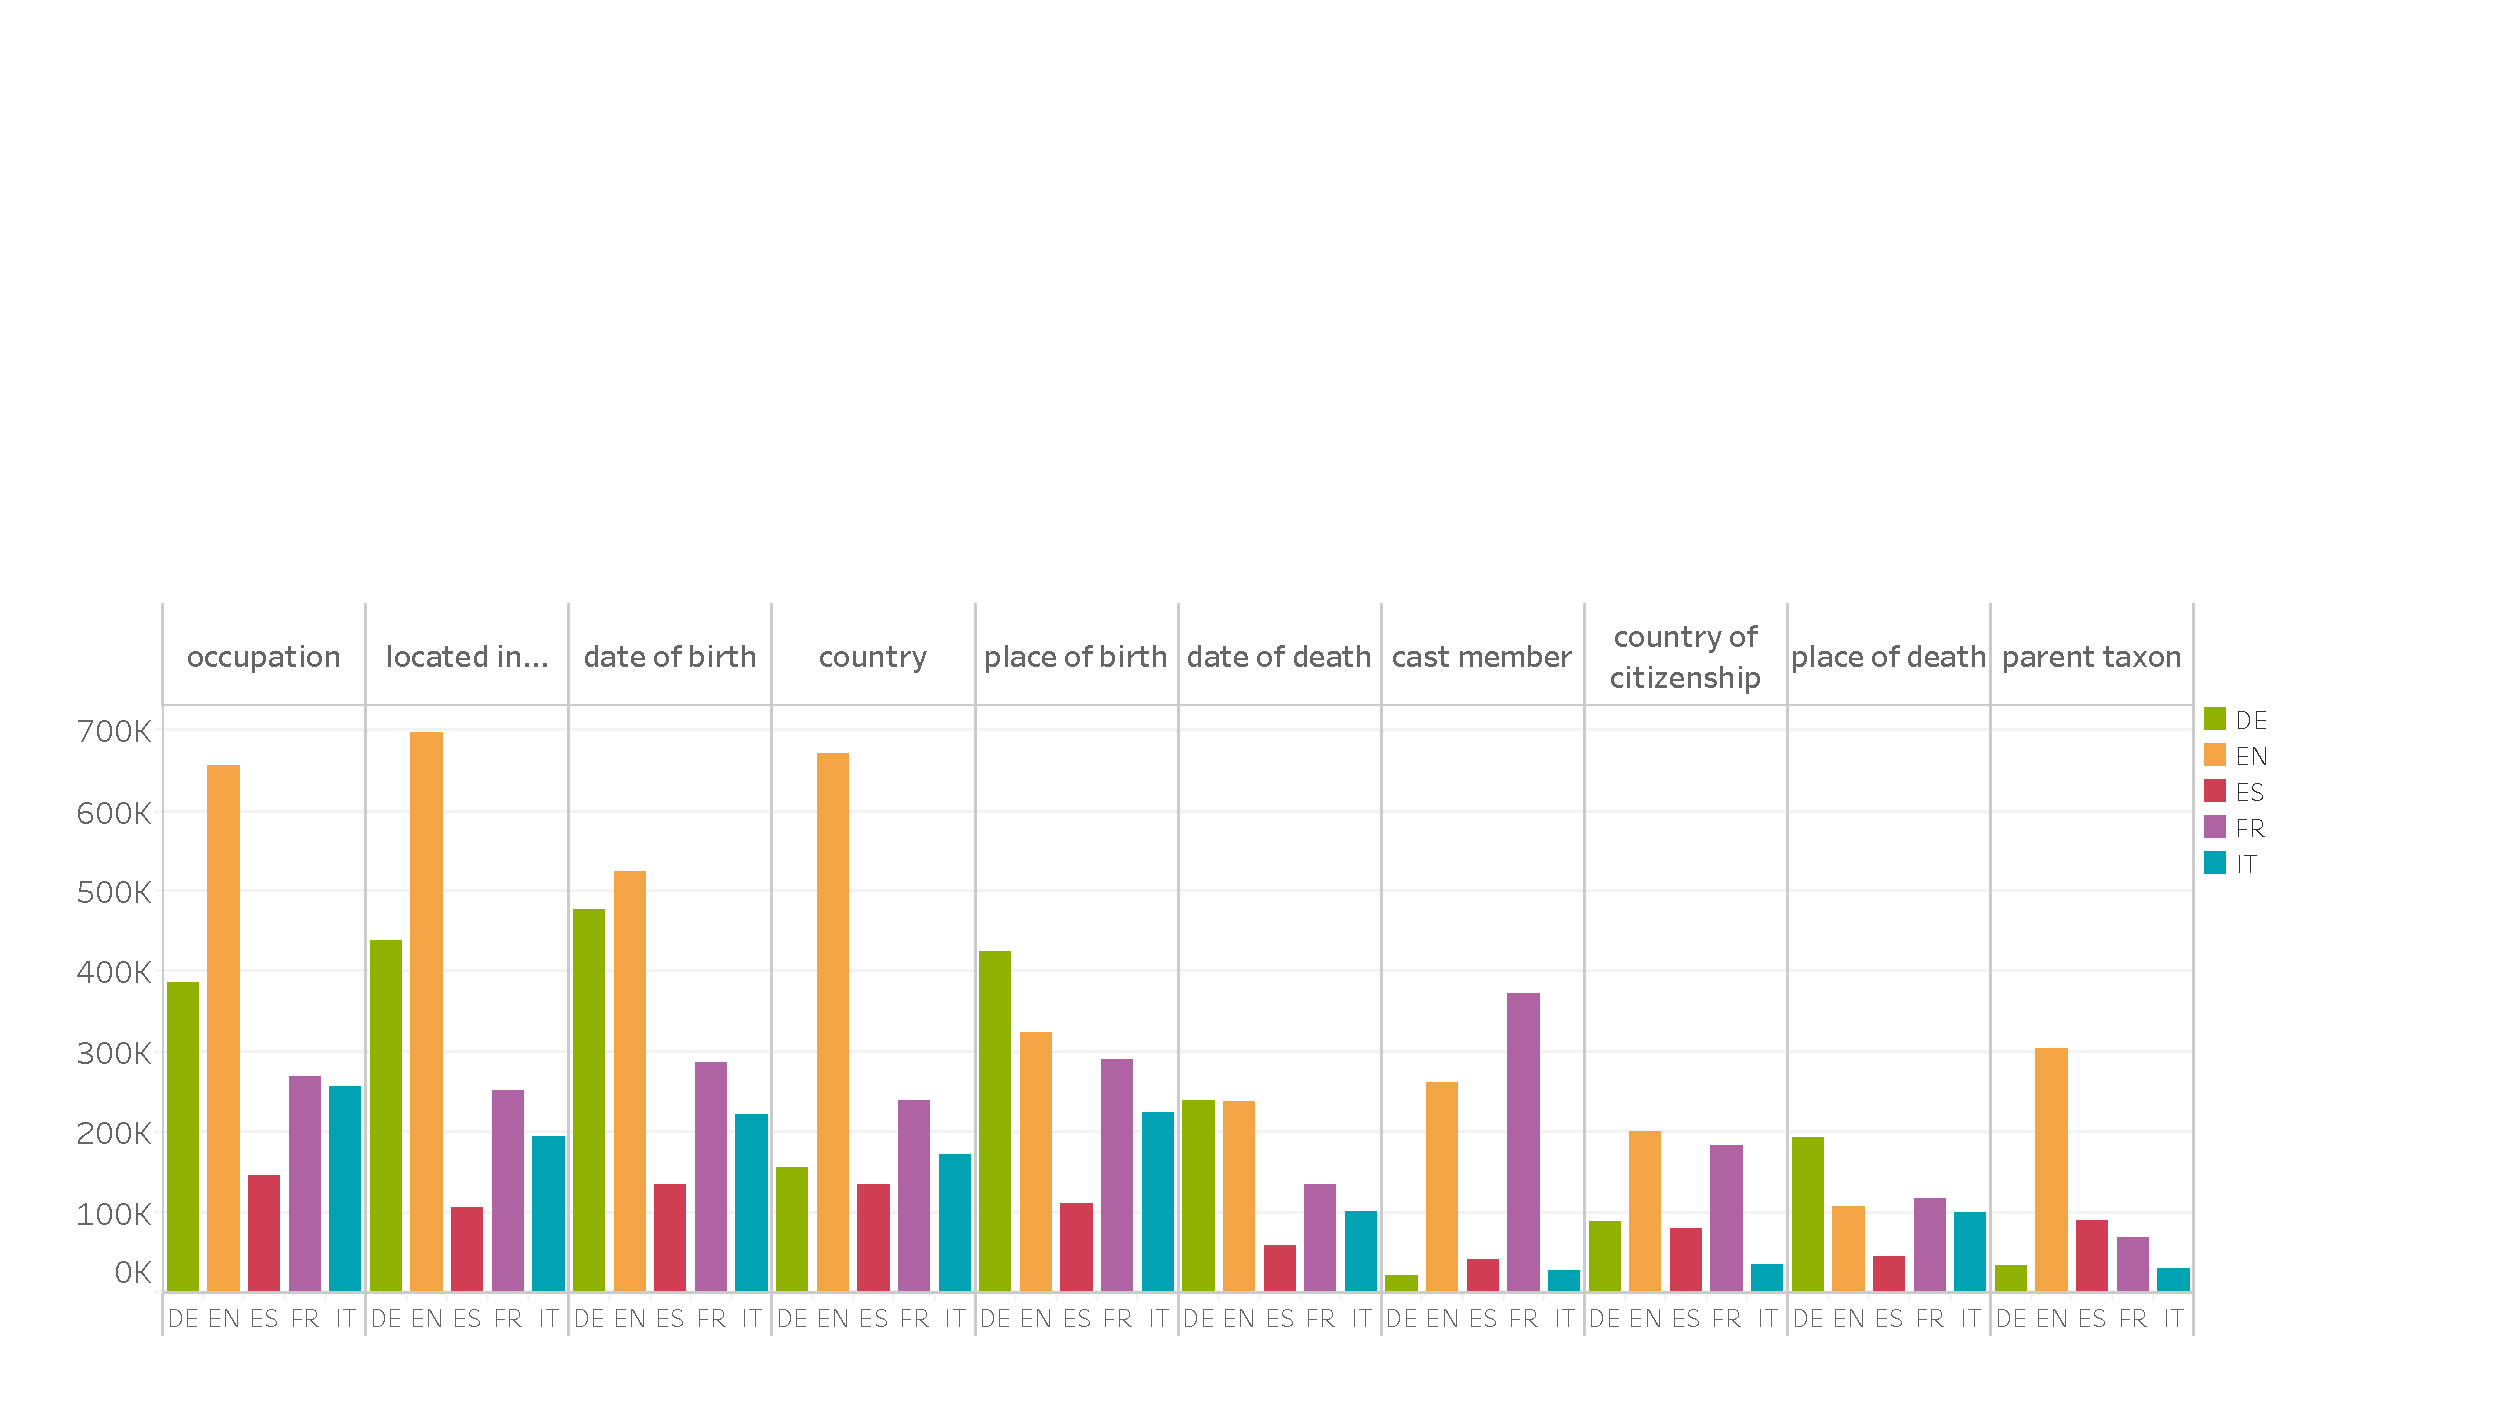
\includegraphics[width=\textwidth]{images/count_examples-property_per_language_wide.pdf}
\caption{The number of triples for the top 10 properties in each language.}
\label{fig:top_10}
\end{figure}


\begin{figure}[h!]
\centering
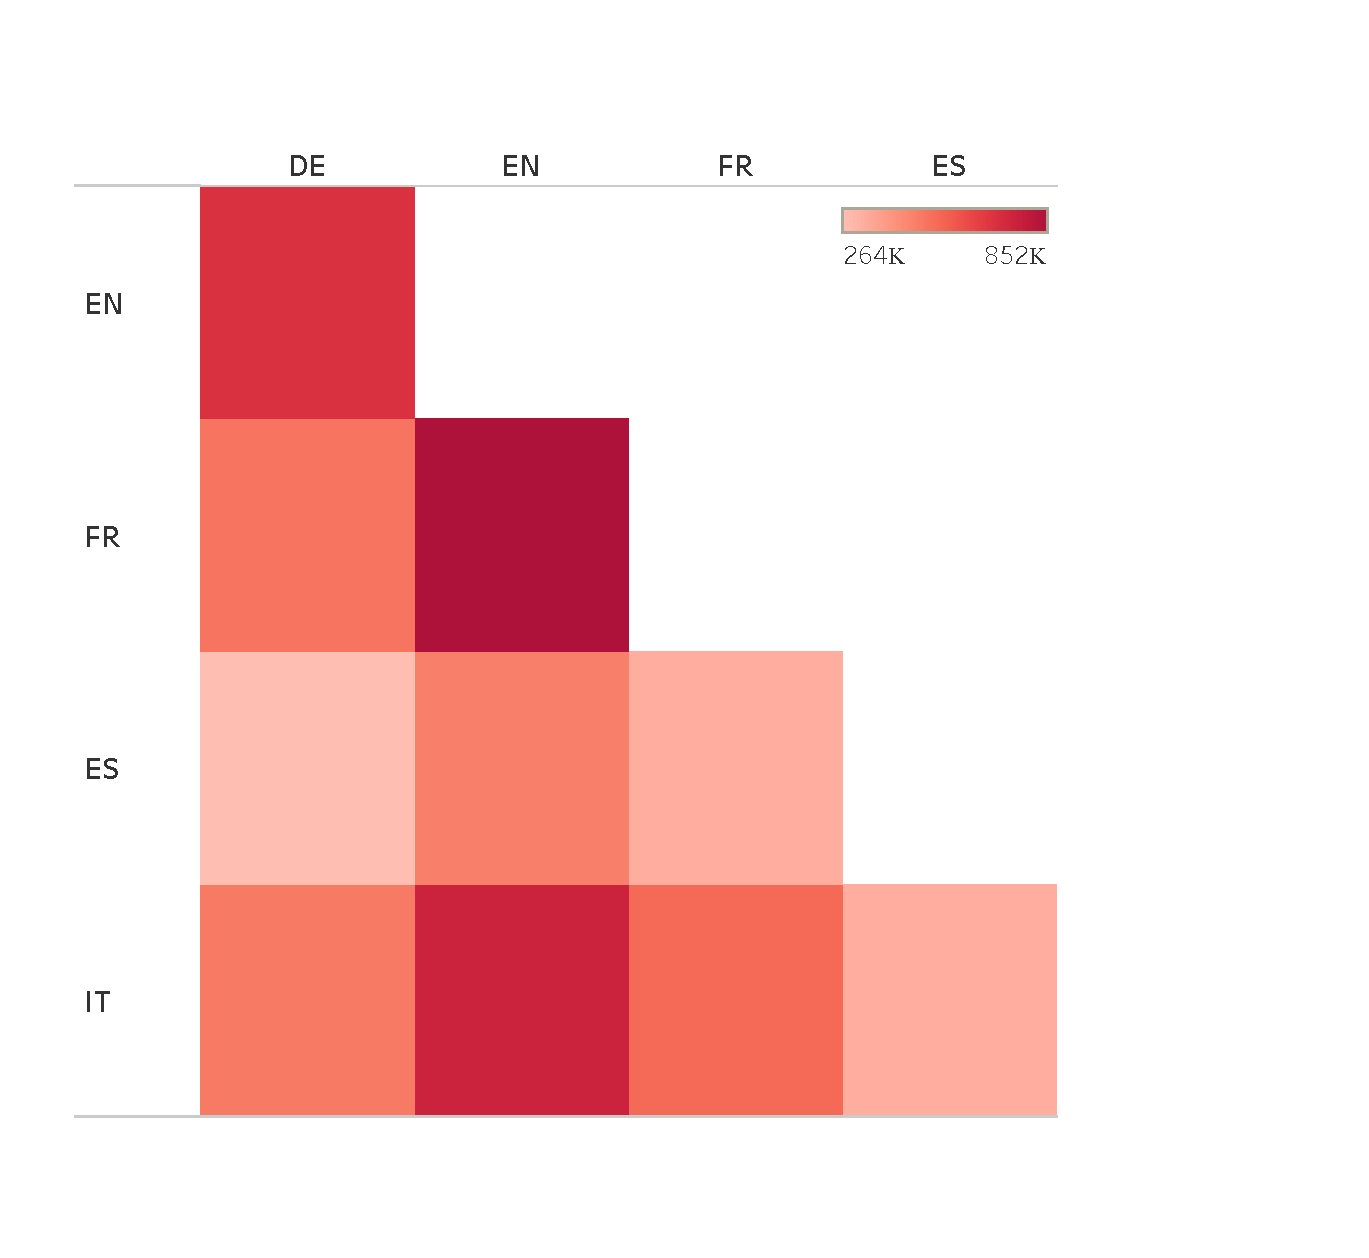
\includegraphics[width=0.4\textwidth]{images/intersection_percentage_all.pdf}
\caption{The overlap of triples between languages.}
\label{fig:intersection_heatmap}
\end{figure}

% \subsubsection{Context size}
% \paragraph{}
% \newpage
Since we will compare our solution against the one of \cite{levy2017zero}, we computed the average length of the context in out dataset and their dataset. Observe from Table~\ref{tab:addlabel} that in our dataset contexts are longer on average. Also observe that, on average, contexts in test set have more tokens than those in the training or development sets for all languages except Italian.

\begin{table}[h!]
  \centering
    \begin{tabular}{c|c|ccc}
    \toprule
    \multicolumn{1}{r}{} & Lang  & Train & Dev   & Test \\
    \midrule
    \cite{levy2017zero} & EN*    & 29 & 28 & 29 \\
    \midrule
    \multirow{5}[2]{*}{X-WikiRE} & EN    & 30 & 33 & 34 \\
          & ES    & 34 & 46 & 48 \\
          & FR    & 49 & 39 & 42 \\
          & DE    & 29 & 30 & 32 \\
          & IT    & 40 & 35 & 35 \\
    \bottomrule
    \end{tabular}%
    \caption{Average number of tokens in the context.}
  \label{tab:addlabel}%
\end{table}%


